\section{Aufbau und Durchführung}
\subsection{1. Veruchsteil: Elektronen im E-Feld}
  Zunächst wird die Schaltung aus Abbildung \ref{fig:Schaltung1} aufgebaut. Daraufhin muss die Apperatur
  eine Minute lang vorgeheizt werden.
  Danach wird zur Untersuchung der Proportionalität der Verschiebung von $D$ und Ablenkspannung $U_d$ die Ablenkspannung so eingestellt, dass
  der Leuchtfleck auf dem unteren Rand des Koordinatennetzes landet. Dabei muss der Fleck ebenso an der vertikalen Markierung sein, damit die
  Abstände gemessen werden können.
  \begin{figure}[H]
    \centering
    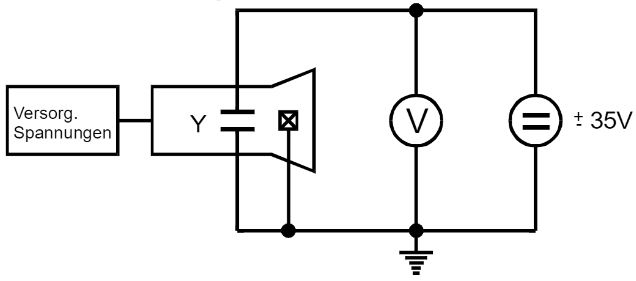
\includegraphics{Text/Bilder/Schaltung1}
    \caption{Schaltung zur Messung der Leuchtfleckverschiebung \cite[85]{sample2}}
    \label{fig:Schaltung1}
  \end{figure}
  Ist dies geschehen, wird die Spannung $U_d$ so variiert, dass der Leuchtfleck einer der nächsten Markierungen erreicht. Dies wird so
  lange durchgeführt, bis das obere Ende des Koordinatengitters erreicht ist.
  Dies wird für 5 verschiedene $U_B$ zwischen $210$ und $\SI{350}{V}$ durchgeführt.
\\
  Nachdem die erste Messung beendet ist, wird die Schaltung aus Abbildung \ref{fig:Schaltung2} aufgebaut.
  Ist dies getan, wird die Frequenz der Sägezahnspannung solange variiert, bis stehende Bilder auf dem Leuchtschirm zu sehen sind.
  \begin{figure}[H]
    \centering
    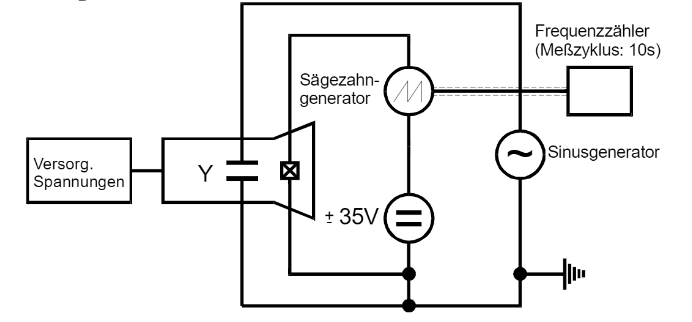
\includegraphics{Text/Bilder/Schaltung2}
    \caption{Schaltbild eines Kathodenstrahloszillographen \cite[85]{sample2}}
    \label{fig:Schaltung2}
  \end{figure}
  Dies ist der Fall, wenn die Frequenzen der Spannungen ein rationales Verhältnis bilden.
  Die Fälle $n \nu_\text{Sä}=\nu_\text{si}$ für $n \in {\frac{1}{2}, 1, 2, 3}$ werden realisiert.
  Die Amplitude und Frequenz werden jeweils gemessen.

\subsection{2. Veruchsteil: Elektronen im B-Feld}

  In diesem Versuchsteil befindet sich die Kathodentrahlröhre im Zentrum eines Helmholzspulenpaar. Dieses bleibt zunächst ausgeschaltet.
  Zu Beginn der Messung wird die Kathodenstrahlröhre so gedreht, dass sie in Richtung der Horziontalkomponente des Erdmagnetfeldes zeigt.
  Es wird als Beschleunigungsspannung zunächst $\SI{250}{V}$ angelegt.
  Nun wird der Leuchtfleck mithilfe eines elektrischen Feldes auf die obere oder untere Seite des Leuchtschirms gelegt.
  Ist dies geschehen, wird das Helmholzspulenpaar eingeschaltet und die dort angelegte Stromstärke erhöht, sodass die Verschiebung
  $D$ in Abhängigkeit von $I$ gemessen werden kann. Die Stromstärke wird solange erhöht, bis das jeweils andere Ende des Leuchtschirms erreicht wird.
  Die Messung wird für $U_B= \SI{400}{V}$ wiederholt.
\\
  In der letzten Messung wird zunächst die Position des Leuchtflecks bei ausgeschalteten Helmholzspulenpaar notiert.
  Es dabei wird eine möglichst niedrige Beschleunigungsspannung gewählt.
  Daraufhin wird die Kathodenstrahlröhre in Ost-West-Richtung gedreht  und der Leuchtpunkt mithilfe eines Magnetfeldes in seine Ursprüngliche Position
  zurückversetzt und die benötigte Stromstärke notiert.
  Zuletzt wird noch der Inklinationswinkel $\varphi$ bestimmt. Das ist der Winkel zwischen Horizontalebene und der Richtung
  des Erdfeldes.
  Dafür wird ein Inklinatorium so gedreht, dass seine horizontale Drehachse parallel zur Magnetnadel ist.
  Danach wird der Teilkreis um 90° in vertikale Richtung gedreht und der Winkel $\varphi$ abgelesen.
